\pdfoutput=1
\documentclass[conference]{IEEEtran}
\IEEEoverridecommandlockouts
\usepackage{graphicx}
\usepackage{amsmath}
\usepackage{booktabs}
\usepackage{siunitx}
\usepackage{tikz}
\usetikzlibrary{positioning,arrows.meta,fit,calc}
\usepackage[hidelinks]{hyperref}
\hypersetup{pdftitle={Is Hardware Offload Enough? Energy, Timing, and Scheduling of a Video Analytics Pipeline on the Raspberry Pi 4}, pdfauthor={Yazeed Alzughaibi}, pdfkeywords={embedded systems, hardware offload, video processing, energy, DVFS, rate-monotonic scheduling, Raspberry Pi}}
\usepackage{xcolor}
\sisetup{detect-all, group-minimum-digits=4}

\definecolor{codec}{HTML}{2a78d6}
\definecolor{cpu}{HTML}{8a8984}

\begin{document}

\title{Is Hardware Offload Enough? Energy, Timing, and Scheduling of a Video Analytics Pipeline on the Raspberry Pi~4}

\author{\IEEEauthorblockN{Yazeed Alzughaibi}
\IEEEauthorblockA{Department of Electrical and Computer Engineering\\
King Abdulaziz University, Jeddah, Saudi Arabia\\
yazeedmalzughaibi@gmail.com}}

\maketitle

\begin{abstract}
Single-board computers ship with hardware video codecs, and the usual advice for a video pipeline with deadlines is to use them. We test that advice on a Raspberry~Pi~4 running a 720p decode--detect--overlay--encode pipeline with a person detector on every tenth frame. Moving decoding and encoding to the hardware codec raises sustained throughput from 18 to 30~frames/s. At equal work (15~frames/s) it cuts CPU time per frame by \SI{52}{\percent}, but outlet energy per frame, measured in one session, by only about \SI{16}{\percent}. Lower CPU time did not mean lower latency: in the way this application collects encoder output, each hardware-encoded packet was retrieved one or two frames after submission, so at 15~frames/s the median time from a frame's release to its encoded packet was \SI{148}{\milli\second} against \SI{72}{\milli\second} in software. With detection moved to a separate worker on one core at 15~frames/s, every hardware-mode frame-task and detection job met its CPU deadline under rate-monotonic priorities, with and without competing load, below an idealized response-time estimate; under the default Linux policy, competing load made every frame-task job late. Smaller findings concern slow CPU access to decoder buffers and the frequency governor.
\end{abstract}

\begin{IEEEkeywords}
embedded systems, hardware offload, video processing, energy, DVFS, rate-monotonic scheduling, Raspberry Pi
\end{IEEEkeywords}

\section{Introduction}

A small board that watches a camera, finds people, and streams the annotated video is a common embedded workload. On a Raspberry~Pi~4 the decoding and encoding can run on the CPU or on a dedicated video block, and the intuition is that the hardware codec should free the CPU, save energy, and make deadlines easier to meet.

We test that intuition by measurement: one pipeline with a software and a hardware codec path, a deadline for every frame, and repeated, balanced runs. The headline result agrees with the intuition; several details do not, and some would be easy to miss.

Our contributions are:
\begin{itemize}
\item A same-board comparison of software and hardware codec paths that separates throughput, CPU-task deadlines, and encoded-output latency, with CPU time and outlet power at equal work (Section~\ref{sec:offload}).
\item A measurement of what reading the hardware decoder's output costs the CPU (Section~\ref{sec:access}).
\item A frame-level comparison of the \texttt{ondemand} and \texttt{performance} governors (Section~\ref{sec:governor}).
\item A single-core version comparing an idealized fixed-priority analysis with measurement, and rate-monotonic with default Linux scheduling under competing load, with every detection job accounted for (Section~\ref{sec:sched}).
\end{itemize}
The scripts, raw logs, analysis code, and a manifest mapping every reported number to its runs and the command that computes it are available at \url{https://github.com/YazeedZee/ee654-pi-energy}.

\section{Background and Related Work}

\textit{Hardware codecs.} The Raspberry~Pi~4's video block decodes and encodes H.264. Linux exposes it as a memory-to-memory V4L2 device, which FFmpeg wraps as \texttt{h264\_v4l2m2m}~\cite{ffmpeg}. Frames come back in buffers shared with the hardware.

\textit{Frequency scaling.} Real-time dynamic voltage and frequency scaling (DVFS) work often assumes execution time scales inversely with frequency~\cite{pillai2001}; memory-bound work and high static power weaken that trade-off, so racing to idle can be as efficient as slowing down~\cite{miyoshi2002,lesueur2010}.

\textit{Fixed-priority scheduling.} For periodic tasks on one processor, rate-monotonic (RM) priority assignment gives shorter periods higher priority. The Liu and Layland bound $U \le n(2^{1/n}-1)$ (0.828 for two tasks) is a sufficient test~\cite{liu1973}; when every period divides the longer ones (harmonic periods), RM schedules any such task set with $U \le 1$. Response-time analysis (RTA) gives the worst-case response of each task from bounds on the execution times~\cite{joseph1986,audsley1993}. The simplified models used here assume independent, preemptible tasks that do not suspend themselves. Linux implements fixed priorities as \texttt{SCHED\_FIFO}; its default policy, \texttt{SCHED\_OTHER}, is a fair-share scheduler, implemented since kernel~6.6 by Earliest Eligible Virtual Deadline First (EEVDF)~\cite{stoica1995,eevdf}, to which the analysis does not apply. Tasks that wait for an accelerator are \emph{self-suspending}, which complicates analysis~\cite{chen2019}.

\textit{Related work.} Hardware and software decoding energy has been compared before, e.g., for HEVC~\cite{khernache2021}, and a low-cost transcoding cluster has been built around the Raspberry~Pi's hardware codec~\cite{liu2018vcc}. Slow CPU access to Raspberry~Pi direct-memory-access (DMA) buffers has been reported, e.g., for camera buffers on a Pi~4~\cite{picam740}. Marasini and Zhou cap the clock of a passively cooled Raspberry~Pi~5 running a detector and report that a fixed maximum clock throttles heavily without a fan~\cite{marasini2026}. We found no study measuring codec offload, buffer access, governor, and scheduling policy together; ours is a reproducible case study of their interaction on one board, not a new mechanism.

\section{Platform and Method}
\label{sec:method}

\textit{Platform.} All runs use one Raspberry~Pi~4 Model~B (rev.~1.4, \SI{4}{\giga\byte}, four Cortex-A72 cores, 600--1800~MHz in 100~MHz steps) with Raspberry~Pi~OS (Debian~13), kernel~6.18.60 (\texttt{PREEMPT}, not \texttt{PREEMPT\_RT}), FFmpeg~7.1.5, PyAV~14.2, and OpenCV~4.10. The board boots to a text console with non-essential services disabled. It has heatsinks and a \SI{5}{\volt} fan, no case, and a USB-C charger. The firmware's under-voltage and throttle flags were clear in every sample of the runs behind Sections~\ref{sec:offload}, \ref{sec:governor} and~\ref{sec:sched}. The earlier diagnostic runs of Section~\ref{sec:access} were made on a weaker USB supply; Section~\ref{sec:access} states which of them were affected. Frequency is left to the default \texttt{ondemand} governor unless stated.

\textit{Pipeline v1.} Fig.~\ref{fig:pipeline} shows the pipeline. A frame is decoded from H.264, converted from YUV to BGR, annotated with the latest boxes, converted back to YUV, and encoded at \SI{4}{\mega\bit\per\second}. Every $N=10$ frames a person detector (MobileNet-SSD~\cite{howard2017,liu2016} on a $300{\times}300$ input through OpenCV's DNN module) runs first; in pipeline~v1 it runs inline, so that frame waits for it. At 30 and 15~frames/s this is 3 and 1.5 detections per second. In \emph{software mode} decoding and encoding run on the CPU (FFmpeg's H.264 decoder and \texttt{libx264}, preset \texttt{veryfast}, tune \texttt{zerolatency}); in \emph{hardware mode} both use \texttt{h264\_v4l2m2m}. Everything else is identical. Frame $i$ is \emph{released} at $t_0 + iT$, the scheduled start of its processing iteration, as if a camera delivered it then, and its deadline is one period later. The iteration starts at release or when the previous one ends, whichever is later, and asks the decoder for its next frame; the decoder is fed compressed packets from memory whenever it has none ready, so packets enter it ahead of their release, and time they spend inside the decoder before that is not measured. Late frames are not dropped, so a pipeline that cannot keep up builds a growing backlog. Pipeline~v2, used only in Section~\ref{sec:sched}, moves the detector into a separate worker thread.

\begin{figure*}[t]
\centering
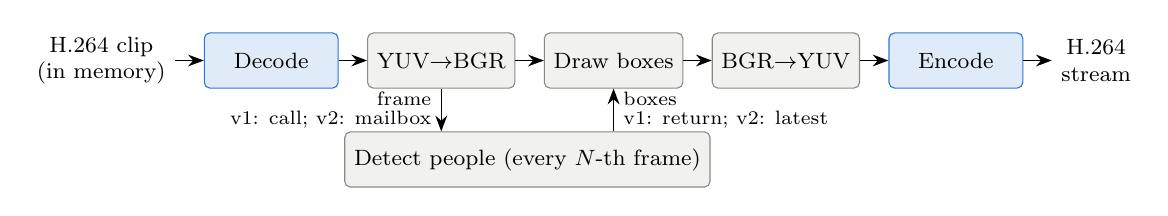
\begin{tikzpicture}[
  st/.style={draw, rounded corners=2pt, minimum height=7mm, minimum width=17mm, align=center, font=\footnotesize, line width=0.4pt},
  co/.style={st, fill=codec!15, draw=codec},
  cp/.style={st, fill=cpu!12, draw=cpu},
  ar/.style={-{Stealth[length=2mm]}, line width=0.5pt},
  node distance=3.6mm]
\node[font=\footnotesize, align=center] (src) {H.264 clip\\(in memory)};
\node[co, right=of src] (dec) {Decode};
\node[cp, right=of dec] (bgr) {YUV$\rightarrow$BGR};
\node[cp, right=of bgr] (ovl) {Draw boxes};
\node[cp, right=of ovl] (yuv) {BGR$\rightarrow$YUV};
\node[co, right=of yuv] (enc) {Encode};
\node[font=\footnotesize, align=center, right=of enc] (out) {H.264\\stream};
\node[cp, below=9mm of $(bgr)!0.5!(ovl)$, minimum width=40mm] (det) {Detect people (every $N$-th frame)};
\draw[ar] (src) -- (dec); \draw[ar] (dec) -- (bgr); \draw[ar] (bgr) -- (ovl); \draw[ar] (ovl) -- (yuv); \draw[ar] (yuv) -- (enc); \draw[ar] (enc) -- (out);
\draw[ar] (bgr.south) -- node[left, font=\scriptsize, align=right]{frame\\[-1pt]v1: call; v2: mailbox} (bgr.south |- det.north);
\draw[ar] (ovl.south |- det.north) -- node[right, font=\scriptsize, align=left]{boxes\\[-1pt]v1: return; v2: latest} (ovl.south);
\end{tikzpicture}
\caption{The pipeline. Blue stages run on the hardware codec in hardware mode and on the CPU in software mode; gray stages always run on the CPU. In pipeline~v1 (Sections~\ref{sec:offload}--\ref{sec:governor}) the detector is called inline; in pipeline~v2 (Section~\ref{sec:sched}) it is a separate worker fed every $N$-th processed frame through a one-slot mailbox.}
\label{fig:pipeline}
\end{figure*}

\textit{Input.} The input is the \texttt{pedestrian\_area} sequence from the Xiph test-media collection~\cite{xiph} (people walking, static camera), re-timed to 30~frames/s, scaled to 720p, and encoded with \texttt{libx264} (High profile, CRF~20, one-second group of pictures (GOP)). The 375-frame clip is loaded into memory before each run and looped, so storage does not affect timing.

\textit{Timing metrics.} Each stage is timed per frame with a monotonic clock. A frame's \emph{frame-task response} runs from its release to the end of the CPU's work on it, when the frame has been submitted to the encoder; the frame \emph{misses} if that exceeds one period. This is the job completion that scheduling analysis describes, not end-to-end latency: codecs decouple input from output~\cite{ffmpeg}, so the call that submits frame $i$ may return packets of earlier frames. Only the bytes each encoder call returned were logged, so we \emph{reconstruct} which call returned each frame's packet: assuming one packet per frame in submission order (neither encoder uses B-frames), the $k$-th call that returned output carried frame $k$. For the hardware encoder, the alignment of every key frame after the first with a large returned packet, in every run, was consistent with this mapping, but packet identities were not logged; the software encoder never returned an empty call, so its lag is zero throughout. We report the \emph{encoder output lag} in frames and the \emph{reconstructed packet-retrieval latency}, from release to the end of the call that returned the packet: an upper bound on when the packet was ready, describing this application's retrieval rather than the encoder's processing time. Neither includes decoder buffering. A frame's \emph{service time} runs from the start of its first stage to the end of its last; for pipeline~v1 we report a \emph{load factor}, mean service time over the period. CPU time comes from per-process (v1) or per-thread (v2) accounting and can exceed service time, because the codecs and OpenCV run several threads. For pipeline~v2 we use the utilization $U=\sum C_i/T_i$. A sampler reads the ARM clock, temperature, and throttle flags every \SI{0.5}{\second}; the pipeline logs the cpufreq frequency per frame.

\textit{Power.} Power is read from a low-cost plug-in AC energy meter (MECHEER) between the outlet and the charger, so it includes the charger's losses and the fan. The meter displays \SI{0.1}{\watt} steps and updates about once per second; its manual states no accuracy. Readings were taken by hand: the typical value per run for the equal-work comparison, and every value shown at about \SI{5}{\second} intervals for the governor comparison. Readings within a run are not independent (the display aliases with the detector's bursts), so the run is our unit of replication, and we compare only conditions measured in the same session.

\textit{Protocol.} Conditions run in balanced order (A--B--B--A) with \SI{30}{}--\SI{60}{\second} idle gaps. Runs last \SI{90}{}--\SI{180}{\second}, the first 2--\SI{3}{\second} are excluded, and every condition was run at least twice. This protocol applies to the principal comparisons (Sections~\ref{sec:offload}, \ref{sec:governor}, and~\ref{sec:sched}); the diagnostic runs of Section~\ref{sec:access} (\SI{20}{\second} pipeline runs and a 150-frame microbenchmark) are exceptions described there. At equal work, throughput, CPU time per frame, and load factor agreed within \SI{1.5}{\percent} across eight runs per mode in four sessions; miss ratios and power varied more and are given as ranges. Platform state is recorded with every run.

\section{Offloading at the System Level}
\label{sec:offload}

\textit{Throughput and deadlines at 30 frames/s.} The software pipeline cannot keep up: it processes 17.8--17.9~frames/s at a load factor of 1.66, and every frame misses its deadline. The hardware pipeline sustains 30.0~frames/s at a load factor of 0.86; decoding falls from 13.4 to \SI{0.3}{\milli\second} per frame and encoding from 22.9 to \SI{1.6}{\milli\second}. Throughput is not deadline compliance, though. Each detection call takes about \SI{110}{\milli\second} inline, so the frame task misses its deadline for \SI{71}{\percent} of hardware-mode frames, and the hardware encoder's packets are retrieved one frame after submission early in each run and two frames after it from then on (software: in the same call), so no frame's packet is retrieved within one period (median 125--\SI{129}{\milli\second}). This is a throughput result, not a real-time one.

\begin{figure}[t]
\centering
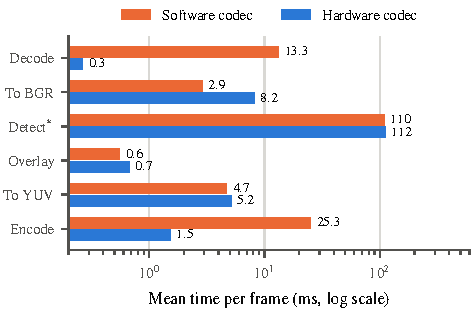
\includegraphics[width=\columnwidth]{figs/stages.pdf}
\caption{Mean time per frame of each stage at 15~frames/s, pipeline~v1 (two runs per mode, one session). $^{*}$Detection runs on one frame in ten and is shown amortised per frame; one call takes 110--\SI{112}{\milli\second} in either mode.}
\label{fig:stages}
\end{figure}

\textit{Equal work.} At 30~frames/s the hardware pipeline does 70\% more work, so we compare energy at 15~frames/s, which both modes sustain (Fig.~\ref{fig:stages}, Table~\ref{tab:equal}). Hardware mode uses \SI{70}{\milli\second} of CPU per frame against \SI{145}{\milli\second}, a \SI{52}{\percent} reduction, at a bitrate 3--\SI{3.5}{\percent} lower. The frame task still misses for \SI{20}{}--\SI{21}{\percent} of hardware-mode and \SI{52}{}--\SI{54}{\percent} of software-mode frames, because detection runs inline. Measured to the reconstructed retrieval of each frame's packet, the order reverses: the median is \SI{148}{\milli\second} in hardware mode, where the lag grew from one frame to two once per run, always at the call after an encoder key frame (in 6 of 8 runs the first key frame after the 375-frame clip first looped, so the input loop may play a part), against \SI{72}{\milli\second} in software mode. In this pipeline, offloading saved CPU time, not latency. The hardware run also ran cooler: in one matched pair of runs that started at 34.1 and \SI{34.6}{\celsius}, it ended at \SI{36.9}{\celsius} against \SI{43.5}{\celsius} after \SI{180}{\second}.

\begin{table}[t]
\caption{Equal work: pipeline v1 at 15 frames/s, $N=10$}
\label{tab:equal}
\centering
\setlength{\tabcolsep}{3.5pt}
\begin{tabular}{@{}lccc@{}}
\toprule
 & Software & Hardware & Change \\
\midrule
\multicolumn{4}{@{}l}{\textit{Four sessions, two runs per mode each}} \\
CPU cores in use & 2.17--2.18 & 1.04--1.06 & $-52\%$ \\
CPU time per frame (ms) & 145 & 70 & $-52\%$ \\
Load factor & 0.87 & 0.41 & \\
Frame-task deadline misses & 52--54\% & 20--21\% & \\
Encoder output lag (frames) & 0 & 1, then 2 & \\
Packet retrieval, median (ms)$^{\dagger}$ & 70--75 & 148 & \\
Encoded bitrate (Mb/s) & 4.05--4.07 & 3.93 & $-3$ to $-3.5\%$ \\
\midrule
\multicolumn{4}{@{}l}{\textit{One session (two runs per mode), outlet power by hand}} \\
Wall power (W; idle 3.6) & $\approx$6.3 & $\approx$5.3 & $-1.0$~W \\
Energy/frame, total (J) & $\approx$0.42 & $\approx$0.35 & $\approx-16\%$ \\
Energy/frame, above idle (J) & $\approx$0.18 & $\approx$0.11 & $\approx-37\%$ \\
\bottomrule
\multicolumn{4}{@{}p{0.97\columnwidth}@{}}{\footnotesize $^{\dagger}$Release to reconstructed retrieval of the frame's encoded packet; frame-task misses end at encoder submission.} \\
\end{tabular}
\end{table}

\textit{Energy.} The wall meter tells a more modest story. In the one session where we read it, the board idled at \SI{3.6}{\watt}, the software pipeline drew about \SI{6.3}{\watt}, and the hardware pipeline about \SI{5.3}{\watt}, with both software runs above both hardware runs. Power above idle fell by about \SI{37}{\percent} and total energy per frame by about \SI{16}{\percent}, because more than half of the software pipeline's power is the idle level both modes pay. These are estimates from an uncalibrated meter, including the charger and fan, so we trust the direction more than the size. Such a gap between system and component savings is not new~\cite{khernache2021}.

\textit{Cooling.} Without the fan (case on), four cores at full load make the firmware throttle the clock, at times to \SI{600}{\mega\hertz}. The pipeline is lighter: in a separate fanless session its 30~frames/s runs ended at 68--\SI{72}{\celsius} against 44--\SI{45}{\celsius} with the fan, the load factor changed by 1--\SI{4}{\percent}, and no run throttled.

\section{The Frame-Access Trap}
\label{sec:access}

Our first hardware pipeline was \emph{slower} than the software one. It converted each decoded frame to BGR directly from the decoder's buffer, and in the one pair of runs of that session without under-voltage throttling (detection every third frame, \SI{20}{\second} each) it managed 5.3~frames/s against 11.8 for software. The decode and encode stages were fast; the conversion took \SI{143}{\milli\second} per frame against \SI{4}{\milli\second} in software mode.

To find the cause, we timed three ways of getting a decoded 720p frame into BGR form, over 150 frames: a bulk copy of the frame's planes into ordinary memory; a conversion of that copy with OpenCV; and the direct conversion the pipeline used, libswscale through PyAV, reading straight from the decoder's buffer (Fig.~\ref{fig:access}). Bulk-copying a hardware-decoded frame is 2.5 times slower than copying a software-decoded one (595 against \SI{1483}{\mega\byte\per\second}), so the decoder's buffers are slower for the CPU to read, but only moderately. The direct conversion, however, takes \SI{138}{\milli\second} from a hardware-decoded frame against \SI{3.9}{\milli\second} from a software-decoded one: the same routine on the same frame size runs 35 times slower. Copying first and then converting takes \SI{4.4}{\milli\second}.

\begin{figure}[t]
\centering
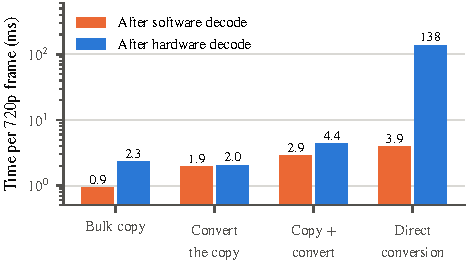
\includegraphics[width=\columnwidth]{figs/frame_access.pdf}
\caption{Getting one decoded 720p frame into BGR form (median of 150 frames, diagnostic session). ``Direct conversion'' uses libswscale on the decoder's buffer; ``convert the copy'' uses OpenCV on a copy in ordinary memory.}
\label{fig:access}
\end{figure}

This diagnostic has two weaknesses. First, the copy-then-convert path used a different routine (OpenCV) from the direct path (libswscale), so the ratio $137.97/4.36\approx31.6$ mixes the copy with the change of routine, and the routines' similar speed on ordinary memory says nothing about the decoder's memory. Second, it ran on the weaker supply with no clock trace, after under-voltage and throttling had occurred that boot. Pipeline~v2 (Section~\ref{sec:sched}), which copies first and converts with libswscale, took \SI{12.2}{\milli\second} for this step in hardware mode (\SI{7.4}{\milli\second} in software mode), but in another session, on another supply and on one core, so the copy's effect is not isolated; we did not run the paired comparison that would isolate it.

What the evidence does show is that the same routine was 35 times slower on the hardware decoder's buffer than on ordinary memory, while a bulk copy of that buffer was only 2.5 times slower. One unverified explanation is that the buffers are mapped without CPU caching, so a conversion's many small reads each pay a full memory access while a bulk copy reads in long bursts; slow CPU access to Raspberry~Pi DMA buffers has been reported before~\cite{picam740}. All other results copy first; even so, the hardware path pays \SI{8.2}{\milli\second} for this stage in pipeline~v1 against \SI{2.9}{\milli\second} in software.

\section{The Frequency Governor}
\label{sec:governor}

At 15~frames/s the hardware pipeline leaves the CPU lightly loaded, and the \texttt{ondemand} governor responds by lowering the clock, briefly, to 700--\SI{800}{\mega\hertz}; the software pipeline never triggered a dip. We ran four trials in balanced A--B--B--A order: \texttt{ondemand}, \texttt{performance}, \texttt{performance}, \texttt{ondemand}. The \texttt{performance} governor requests the maximum frequency of \SI{1.8}{\giga\hertz}. Table~\ref{tab:gov} summarizes the detection frames, the pipeline's longest.

\begin{table}[t]
\caption{Governor runs: hardware mode, 15 frames/s, in run order. Service times (ms) of the 177 detection frames per run}
\label{tab:gov}
\centering
\footnotesize
\setlength{\tabcolsep}{2.6pt}
\begin{tabular}{@{}llcccccc@{}}
\toprule
Run & Governor & Low clk & Median & p99 & Max & \# $>$145 & Power (W) \\
\midrule
1 & \texttt{ondemand} & 7\% & 121.6 & 164.3 & 174.6 & 9 & 5.50 \\
2 & \texttt{performance} & 0\% & 121.5 & 138.6 & 142.8 & 0 & 5.12 \\
3 & \texttt{performance} & 0\% & 121.4 & 137.9 & 144.1 & 0 & 5.38 \\
4 & \texttt{ondemand} & 33\% & 125.2 & 143.9 & 147.2 & 1 & 5.09 \\
\bottomrule
\multicolumn{8}{@{}p{0.97\columnwidth}@{}}{\footnotesize Low clock: share of \SI{0.5}{\second} samples below \SI{1.8}{\giga\hertz}. p99: 99th percentile. \# $>$145: number of detection frames longer than \SI{145}{\milli\second}; the threshold was chosen after inspecting the data, just above the largest value under \texttt{performance}. Power: mean of 22--31 hand readings per run.}
\end{tabular}
\end{table}

The medians are nearly the same under both governors, and the tails differ less uniformly than a first look suggests. Under \texttt{performance}, no detection frame exceeded \SI{144.1}{\milli\second}. Under \texttt{ondemand}, run~1 had nine frames above \SI{145}{\milli\second}, up to \SI{174.6}{\milli\second}, and the frame-boundary frequency log shows all nine began at 900--\SI{1100}{\mega\hertz}. Run~4 spent the most time at low clock but had only one such frame, for which the available frequency samples showed \SI{1.8}{\giga\hertz}, and its detection frames that began or ended at low clock were not slower than the rest (median 124 against \SI{125}{\milli\second}). The evidence supports a governor effect on the tail in one of two runs, not a general rule, and frequency samples at frame boundaries and every \SI{0.5}{\second} are too coarse to attribute each slow frame with certainty.

No energy difference was resolved either: the two runs of one governor differ by about \SI{0.4}{\watt}, more than the governors differ, and two runs per governor allow no meaningful test. This is consistent with diminishing returns from frequency scaling on platforms with high static power~\cite{lesueur2010}. For this workload, with a fan, neither \texttt{performance} run had a detection frame above \SI{145}{\milli\second}. That does not carry over to weaker cooling: the governor only requests the maximum clock, the firmware still lowers it when hot or under-powered, and on a passively cooled Raspberry~Pi~5 a fixed maximum clock throttles heavily~\cite{marasini2026}.

\begin{table*}[t]
\caption{One core, 15 frames/s, $N=10$: two runs per column (ranges). Detection jobs counted after a \SI{3}{\second} warm-up; 131 nominal releases per run}
\label{tab:sched}
\centering
\small
\setlength{\tabcolsep}{5pt}
\begin{tabular}{@{}lcccccc@{}}
\toprule
 & \multicolumn{4}{c}{No competing load} & \multicolumn{2}{c}{Two background processes} \\
\cmidrule(lr){2-5}\cmidrule(l){6-7}
 & HW, RM & HW, default & SW, RM & SW, default & HW, RM & HW, default \\
\midrule
Frames/s & 15.0 & 15.0 & 10.7 & 7.9 & 15.0 & 13.6--13.8 \\
Frame-task deadline misses & 0\% & 0\% & 100\% & 100\% & 0\% & 100\% \\
Frame-task response p99 & 23~ms & 41--42~ms & 26~s & 42~s & 23~ms & 7.1--8.4~s \\
$C_f$ mean / max (ms) & 19 / 24 & 19 / 24 & 93 / 116--118 & 95 / 119--120 & 19 / 24 & 18 / 22 \\
$C_d$ mean (ms) & 301--303 & 302--306 & 293--295 & 297--298 & 302--303 & 309--311 \\
$C_d$ max (ms) & 304--305 & 307--310 & 293--295 & 298--299 & 304--305 & 317--321 \\
$U$ with max $C$ & 0.82 & 0.82 & 2.2 & 2.2 & 0.82 & 0.80--0.81 \\
RTA estimate, detection & 498--501~ms & n/a & unsched. & n/a & 497--498~ms & n/a \\
\midrule
Detection jobs handed over & 131 & 131 & 91--92 & 67 & 131 & 118--120 \\
\quad overwritten unstarted & 0 & 0 & 90--91 & 0 & 0 & 48--49 \\
\quad completed (of which after run end) & 131 (1) & 131 (1) & 1 (1) & 67 (0--1) & 131 (1) & 70--71 (1--2) \\
\quad completed on time & 131 & 131 & 0 & 0 & 131 & 0 \\
Detection response max & 445--447~ms & 445--448~ms & 26--27~s & 42.5--42.9~s & 445--447~ms & 8.9--10.0~s \\
\midrule
Encoder output lag (frames) & 2 & 1 & 0 & 0 & 2 & 1 \\
Reconstructed packet retrieval, median & 152~ms & 100--101~ms & 14~s & 23~s & 153~ms & 3.8--4.6~s \\
Box age in video, median / max (frames) & 11--12 / 16--17 & 11 / 16 & none drawn & 8 / 13 & 11 / 16 & 31 / 44 \\
Box age at encoder submission, median & 0.76--0.79~s & 0.78~s & none drawn & 23~s & 0.76~s & 5.8--6.5~s \\
\bottomrule
\multicolumn{7}{@{}p{0.97\textwidth}@{}}{\footnotesize ``n/a'': fixed-priority RTA does not apply to \texttt{SCHED\_OTHER}. Frame-task responses and misses end at encoder submission. ``After run end'': completed after the timed run ended; when a run stops, the worker finishes its current job and any job still in the mailbox. Box age in video: frames between the analysed frame and the frame on which its boxes are drawn (one frame is \SI{66.7}{\milli\second} of video). Box age at encoder submission: from the analysed frame's release to the end of the frame task for the frame showing its boxes. Packet retrieval: reconstructed, see Section~\ref{sec:method}.}
\end{tabular}
\end{table*}

\section{Scheduling on One Core}
\label{sec:sched}

Pipeline~v1 runs detection inline on four cores, which makes classical analysis hard to apply. Pipeline~v2, pinned to one core with one thread for OpenCV and for each codec, splits the work between a periodic \emph{frame task} (decode to encoder submission, $T_f=\SI{66.7}{\milli\second}$ at 15~frames/s) and a frame-triggered \emph{detection worker} with nominal demand every ten frame periods ($T_d=\SI{666.7}{\milli\second}$). When the frame task processes a frame whose index is a multiple of ten, it places a copy in a one-slot mailbox, overwriting any job the worker has not yet taken; each frame draws the latest boxes. Deadlines equal periods, and a detection job's response is measured from its frame's release. Under RM (\texttt{SCHED\_FIFO}) the frame task has priority~80 and the worker~70; the pipeline exits if it cannot set them. The alternative is the default \texttt{SCHED\_OTHER}.

The execution time $C$ of each job is its thread's CPU time. Each run computes the utilization and RTA from the largest $C$ \emph{observed in that same run}: a consistency check, not an independent prediction, and observed maxima are not proven worst-case execution times. We treat the analysis as an idealized reference model; it assumes independent, preemptible, periodic tasks without suspension, whereas here the worker is released by the frame task with some jitter, the threads share a mailbox and Python's interpreter lock, and part of the codec work runs outside them. Within the model the periods are harmonic, so the RM utilization limit is 1, not 0.828. Table~\ref{tab:sched} accounts for every nominal detection job.

\textit{CPU-task schedulability in the tested configuration.} On one core, detection takes about \SI{300}{\milli\second} per call instead of \SI{110}{\milli\second} on four. In hardware mode the frame task needed at most \SI{24.4}{\milli\second}, so in the reference model $U = 24.4/66.7 + 305.3/666.7 \approx 0.82$, below the harmonic limit of 1. RTA iterates $R = C_d + \lceil R/T_f \rceil C_f$ from $R = C_d + C_f$. With the unrounded maxima of run~1, $C_f = 24.421$ and $C_d = \SI{305.345}{\milli\second}$, it gives 329.8, 427.5, 476.3, and \SI{500.7}{\milli\second}, where it stops. The measured worst detection responses were 445--\SI{447}{\milli\second}, below the estimate in every RM run, and no frame-task or detection job missed its deadline. The measured response includes 14--\SI{16}{\milli\second} between a frame's release and the hand-over to the mailbox, a release jitter the model does not include; the estimate held despite it, but the model does not guarantee that it would.

These are deadlines for the CPU work. In every RM run each frame's packet was retrieved two frames after submission, constantly throughout the run, so the reconstructed retrieval latency was about \SI{152}{\milli\second} (at most \SI{158}{\milli\second}); under \texttt{SCHED\_OTHER} without competing load the lag was one frame (about \SI{100}{\milli\second}). These figures describe when this application collected the packets, not how long the encoder needed. We did not determine why the lag depends on the policy; kernel work serving the codec may wait while the real-time threads run. An application with an end-to-end deadline would need this latency in its budget, or a design that collects encoder output as soon as it is ready.

In software mode the frame task alone needs \SI{93}{\milli\second} on average, more than its \SI{66.7}{\milli\second} period, so no policy can help, and the two fail in opposite ways. RM protects the frame task (10.7~frames/s, the most the core allows) and starves the detection worker: it never ran during the run, all but one handed-over job was overwritten, and that one completed after the run stopped. \texttt{SCHED\_OTHER} lets the frame rate fall to 7.9~frames/s; it completed every job it was handed, but only 67 of 131 were handed over, none on time, and \SI{42.4}{\second} of the worst response of \SI{43}{\second} was frame backlog before hand-over. Because jobs are handed over only when frames are processed, an overloaded frame task also lowers the detection demand.

\textit{When the default policy is enough, and when it is not.} We expected \texttt{SCHED\_OTHER} to cause frame misses in the schedulable hardware case. It did not: the frame task sleeps most of each period, and the default scheduler serves a waking task promptly, so with nothing else to run it behaves much like RM. The difference shows in the margin (99th-percentile frame-task response 41--\SI{42}{\milli\second} against \SI{23}{\milli\second}) and becomes decisive when other work shares the core. With two CPU-bound background processes, RM results were unchanged, because ordinary processes cannot preempt real-time ones. Under \texttt{SCHED\_OTHER} the frame task received only a fair share of the core and fell to 13.6--13.8~frames/s, built a backlog until every frame was late (Fig.~\ref{fig:sched}), 48--49 detection jobs were overwritten, and none of the 70--71 completed finished on time. The boxes on a frame came from a frame 31 frames earlier in the video (median; 11 under RM), released 5.8--\SI{6.5}{\second} before that frame reached the encoder (\SI{0.76}{\second} under RM). The reference model does not cover this case, since \texttt{SCHED\_OTHER} provides neither fixed priorities nor isolation from other processes; it was an empirical baseline.

\begin{figure}[t]
\centering
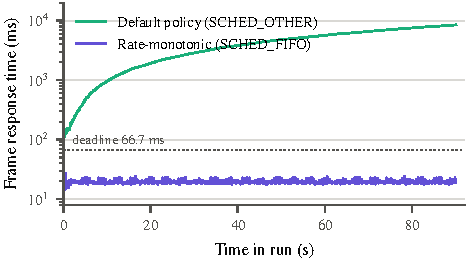
\includegraphics[width=\columnwidth]{figs/sched_bg.pdf}
\caption{Frame-task response times on one core with two background CPU-bound processes, hardware mode. The task set is identical; only the scheduling policy differs, and the response-time analysis applies only to the fixed-priority (RM) case.}
\label{fig:sched}
\end{figure}

\textit{Suspension and blocking.} A frame task waiting for the codec would suspend itself~\cite{chen2019}, and both threads share Python's interpreter lock. Under RM, however, the largest gap between wall-clock service time and CPU time of any frame was \SI{0.01}{\milli\second}, and no frame started more than \SI{0.09}{\milli\second} late, over 5224 frames: no appreciable codec or lock blocking was observed in these runs, consistent with the decoder being fed ahead and packets being collected by later calls. These are observations, not bounds, and work by the video block or kernel threads on other cores is not in $C$.

\section{Limitations}

We used one board, clip, resolution, detector, software encoder preset (\texttt{veryfast}), and a Python pipeline, and did not compare output quality; our claim is that this configured software path misses its deadlines, not that every software path would. Packet retrieval was reconstructed from logged sizes, and decoder buffering was not measured. Power was read by hand from an uncalibrated outlet meter. The scheduling analysis is an idealized model checked against the runs that supplied its observed (not worst-case) execution times, on a kernel without \texttt{PREEMPT\_RT}, without separating interrupt and driver work or recording real-time bandwidth settings. The frame-access diagnostic did not isolate the copy's effect. The governor comparison covers one load level with coarse frequency sampling, and the temperature difference one pair of runs.

\section{Conclusion}

Moving the codec to hardware did what it is expected to do for throughput and CPU time: 30 instead of 18~frames/s, and half the CPU time at equal work. Everything else needed qualification. Hardware mode's CPU work met its deadlines only after detection became a separate, lower-priority worker, and even then, under RM, this application retrieved each frame's encoded packet two frames later. The outlet-energy saving was about a third of the CPU saving. The gain depended on how the CPU read the decoder's output. The default governor coincided with slow frames in one of two runs, for no resolvable energy benefit. And the idealized response-time analysis agreed with measurement under fixed priorities, while the default policy, which it does not cover, failed once other work shared the core. Before trusting an offload, check how the CPU reads the accelerator's buffers, when its output for a frame becomes available, how the governor treats bursty work under the available cooling, and whether the scheduling policy provides what the timing analysis assumes.

\section*{Acknowledgment}
Generative AI was used in this work. Claude (Anthropic) helped write the experiment, pipeline, and analysis scripts, analyse the logs, and draft and revise the text of all sections. ChatGPT (OpenAI) reviewed drafts and suggested related work, which was then checked against the sources. The author designed and ran all experiments, reviewed all content, and takes responsibility for it.

\begin{thebibliography}{99}
\bibitem{ffmpeg} FFmpeg project, ``FFmpeg,'' version 7.1. [Online]. Available: \url{https://ffmpeg.org}
\bibitem{pillai2001} P.~Pillai and K.~G. Shin, ``Real-time dynamic voltage scaling for low-power embedded operating systems,'' in \textit{Proc. 18th ACM Symp. Operating Systems Principles (SOSP)}, 2001, pp.~89--102.
\bibitem{miyoshi2002} A.~Miyoshi, C.~Lefurgy, E.~Van~Hensbergen, R.~Rajamony, and R.~Rajkumar, ``Critical power slope: Understanding the runtime effects of frequency scaling,'' in \textit{Proc. 16th Int. Conf. Supercomputing (ICS)}, 2002, pp.~35--44.
\bibitem{lesueur2010} E.~Le~Sueur and G.~Heiser, ``Dynamic voltage and frequency scaling: The laws of diminishing returns,'' in \textit{Proc. Workshop on Power Aware Computing and Systems (HotPower)}, 2010.
\bibitem{liu1973} C.~L. Liu and J.~W. Layland, ``Scheduling algorithms for multiprogramming in a hard-real-time environment,'' \textit{J. ACM}, vol.~20, no.~1, pp.~46--61, 1973.
\bibitem{joseph1986} M.~Joseph and P.~Pandya, ``Finding response times in a real-time system,'' \textit{The Computer Journal}, vol.~29, no.~5, pp.~390--395, 1986.
\bibitem{audsley1993} N.~Audsley, A.~Burns, M.~Richardson, K.~Tindell, and A.~J. Wellings, ``Applying new scheduling theory to static priority pre-emptive scheduling,'' \textit{Software Engineering Journal}, vol.~8, no.~5, pp.~284--292, 1993.
\bibitem{stoica1995} I.~Stoica and H.~Abdel-Wahab, ``Earliest eligible virtual deadline first: A flexible and accurate mechanism for proportional share resource allocation,'' Old Dominion Univ., Tech. Rep. TR-95-22, 1995.
\bibitem{eevdf} The Linux kernel documentation, ``EEVDF scheduler.'' [Online]. Available: \url{https://docs.kernel.org/scheduler/sched-eevdf.html}
\bibitem{chen2019} J.-J. Chen \textit{et al.}, ``Many suspensions, many problems: A review of self-suspending tasks in real-time systems,'' \textit{Real-Time Systems}, vol.~55, no.~1, pp.~144--207, 2019.
\bibitem{khernache2021} M.~Bey~Ahmed~Khernache, Y.~Benmoussa, J.~Boukhobza, and D.~Menard, ``HEVC hardware vs software decoding: An objective energy consumption analysis and comparison,'' \textit{J. Systems Architecture}, vol.~115, art.~no.~102004, 2021, doi: 10.1016/j.sysarc.2021.102004.
\bibitem{liu2018vcc} P.~Liu, J.~Yoon, H.~R. Kim, and S.~Banerjee, ``VideoCoreCluster: Energy-efficient, low-cost, and hardware-assisted video transcoding system,'' \textit{Wireless Commun. Mobile Comput.}, vol.~2018, art.~no.~7470234, 2018, doi: 10.1155/2018/7470234.
\bibitem{picam740} Raspberry Pi Ltd., \texttt{picamera2} GitHub issue \#740 (discussion of slow CPU copies from camera buffers). [Online]. Available: \url{https://github.com/raspberrypi/picamera2/issues/740}
\bibitem{marasini2026} A.~Marasini and Z.~Zhou, ``Sustainable edge vision via empirically calibrated DVFS: Eliminating thermal throttling on passively cooled hardware,'' arXiv:2609.04705, 2026.
\bibitem{howard2017} A.~G. Howard \textit{et al.}, ``MobileNets: Efficient convolutional neural networks for mobile vision applications,'' arXiv:1704.04861, 2017.
\bibitem{liu2016} W.~Liu \textit{et al.}, ``SSD: Single shot multibox detector,'' in \textit{Proc. European Conf. Computer Vision (ECCV)}, 2016, pp.~21--37.
\bibitem{xiph} Xiph.Org Foundation, ``Xiph.org video test media (derf's collection).'' [Online]. Available: \url{https://media.xiph.org/video/derf/}
\end{thebibliography}

\end{document}
